\documentclass[10pt]{article}

\pagestyle{plain}
\textheight 9in
\textwidth  6.5in
%\footheight 0.0cm
\topmargin  0pt
\headheight 0in
\headsep 0in
\leftmargin 0.0cm
\oddsidemargin  0cm
\def\baselinestretch{1.0}
\parindent 0.0 cm
\parskip   0.2 cm

\newcounter{step}
\newtheorem{theorem}{Theorem}
\newtheorem{proposition}{Proposition}
\newtheorem{corollary}{Corollary}
\newtheorem{definition}{Definition}

\renewcommand{\floatpagefraction}{0.90}
\renewcommand{\topfraction}{0.90}
\renewcommand{\bottomfraction}{0.90}
\renewcommand{\textfraction}{0.10}

\def\thesection{\large{\arabic{section}.}}
\def\thesubsection{\normalsize{\thesection\arabic{subsection}}}
\def\thesubsubsection{\normalsize{\thesection\arabic{subsection}.\arabic{subsubsection}}}
\usepackage{float}
\usepackage[dvips,xetex]{graphicx}
\usepackage{caption}
\usepackage{subcaption}
\begin{document}

\newpage
\thispagestyle{empty}
\begin{center}
{\Large \textbf{Post-Disaster Recovery of Multiple Infrastructures: \\ Coordinating Road and Power Grid Repairs}} \\
\vspace*{0.2cm}
%{\large \textbf{Brian French and Erhan Kutanoglu}} \\
%{\large \textbf{Operations Research and Industrial Engineering Program}} \\
%{\large \textbf{The University of Texas at Austin}} \\
%{\large \textbf{Austin, TX 78712, USA}} \\
%{\large \textbf{BCFrench@utexas.edu, erhank@mail.utexas.edu}} \\
\end{center}

\thispagestyle{empty}
\begin{center}
{\large \bf Abstract}
\end{center}
Both power and road networks sustain major damage in the wake of hurricanes and other natural disasters. Recovery efforts (involving mainly repair of network elements)  should therefore consider the interactions between the two networks. We introduce several coordination frameworks based on the models for both power and road repair and use them to demonstrate the impacts of coordinating repairs. These models are run on several example networks and damage scenarios using IEEE power grid standards to provide computational examples. Results show that a rather simple coordination scheme between two repair agencies based on solving the two models sequentially is quite effective producing repair schedules close to a theoretical lower bound.


{\large \bf Keywords}\\
\vspace*{-12pt}

\vspace*{-12pt}
\section{{\large Introduction}}
\label{sec:ic:intro}
\vspace*{-12pt}

Hurricanes are a growing concern in the operation of power grids in coastal areas. This paper addresses the gap in the literature where previous efforts have not explicitly considered how multiple networks depended on each other. Most notably the post-disaster infrastructure recovery interactions between power grid and road networks. For example, to repair a damaged power grid element, the element must be accessible to the crew attempting to repair it. Moreover, the crew will take time to go from one element to the next to repair, affecting the power grid's performance during recovery. This implies that the road network (how damaged it is and how its recovery is planned) becomes part of the overall recovery efforts. During a hurricane, the road network will sustain substantial damage from flooding and debris on the road surface, which necessitates road grid repairs/clearance as well. To handle the issues of repairing power grids efficiently, both types of repairs (road network and power grid) should be considered jointly. Previous literature does not study this specific interaction as discussed below.
\vspace*{-12pt}
\subsection{\large Existing Literature}
\vspace*{-12pt}
Damage from hurricanes on infrastructure elements is well studied. Both of \cite{WinklerEA2010} and \cite{GuikemaEA2010} have looked at the damage to power grids in varying capacities and methodologies. Damage to the road network is studied more in the context of repairs. \cite{AksuEA2014} addresses concerns of accessibility to locations in the wake of road damage. \cite{DuqueEA2016} focuses their work on the ability to move disaster supplies around.

In the context of power grid repair, literature on this topic comes from two major areas: Network interdiction and work similar to this paper, natural disasters. \cite{SalmeronEA2010} is a paper emblematic of work on interdiction and provides the basis for the linear programming formulation of DC power flow used in this paper.  \cite{NPSMasters} addresses a problem similar to this work, though without addressing travel times. \cite{ArabEA2015} addresses repairs to power grids in the context of resilience. Most similar to this paper is \cite{BentEA2011} in that they consider DC power flow and repair with travel times jointly. The key distinction is that they presume that the road operates under nominal conditions rather than including the repairs of the road elements into the problem.
\vspace*{-12pt}
\section{\large{Model}}
\vspace*{-12pt}
\subsection{Overview}
The problem we consider is how to handle interactions between road and power networks during post-disaster recovery. We consider doing this by solving the problems of the two networks separately to keep runtime tractable and then testing a variety of post processing methods to handle the interactions. This will allow us to capture which interactions are worth the effort to explicitly include and which can be ignored in the name of preserving runtime or simplifying analysis. 
\subsection{Assumptions}
\vspace*{-12pt}
While considering coordinated repairs of road and power networks using the mixed-integer programs below, we assume complete information about infrastructure damage to both networks, complete information about repair times, and no variation in repair times. In the course of modeling the power grid repair problem, we assume that a DC-flow model of operation is close enough to real network behavior to draw useful insights \cite{QiEA2012}. We also assume in the power grid repair model that a minimum spanning tree can approximate the road-network routing between power elements. Here, we take advantage of the fact that the minimum spanning tree provides a lower bound on the traveling salesman problem and therefore the routing portion of the back-to-back repairs of multiple power elements .
\subsection{Road Network Repair Model}
\vspace*{-12pt}
To model the road repair aspect of the problem, we choose to treat it as a problem of routing a crew tasked with clearing debris and flooding from roads. In doing this, damaged roads are not assumed to be totally blocked, but their lengths are merely increased to account for the difficulty traversing them while clearing debris, minor flooding, and the like. This problem is handled by solving a variation of the prize collecting rural postman problem at each time step, representing the shifts that the crew uses during post-disaster recovery. The discrete time based modeling is chosen to match up with both standard shift lengths and the discrete time requirement of the DC power flow based model for the power grid repairs. 

We use the following notation, starting with sets and parameters, followed by decision variables:
\begin{displaymath}
\begin{array}{ll}
T & \mbox{the set of time periods (shifts) over the time horizon, indexed by $t$}\\
N & \mbox{the set of nodes in the graph, representing the intersections of road segments}\\
c_{ij}^t & \mbox{measure of the value of the road segment from node $i$ to node $j$ during period $t$}\\
l_{ij} & \mbox{is the time to traverse the road segment between nodes $i$ and $j$ when everything is working as normal}\\
r_{ij} & \mbox{time to repair the road segment between nodes $i$ and $j$ (hours), including travel time}\\
s^t & \mbox{the length of period $t$ in time units (hours)}\\
o_{ij} & \mbox{initial condition of the road segment between nodes $i$ and $j$}\\
X_{ij}^t & \mbox{binary variable for road segment $ij$ being operational in time $t$}\\
K_{ij}^t & \mbox{binary variable for travel from $i$ to $j$ being in the tour at time $t$}\\
S_{ij}^t & \mbox{length of travel for road segment $ij$ at time $t$}\\
\end{array}
\end{displaymath}

We minimize the total value of non-functioning road segments over the repair horizon. Without loss of generality the objective can be replaced with the repair priority weights for an agency of choice, by modifying the $c_{ij}$s. Then, the road repair model is as follows:
\begin{equation}
	\min \sum_{t \in T}  \sum_{i,j \in N} c_{ij}(1-X_{ij}^t) 
\end{equation}
subject to:
	\begin{eqnarray}
	\sum_{i,j \in N} S_{ij}^t K_{ij}^t \leq s^t, \hspace{6pt} \forall t\in T \\
	S_{ij}^t = \max \{l_{ij}, r_{ij}(1-X_{ij}^t) \}, \hspace{6pt} \forall t\in T, \hspace{5pt} \forall i,j \in N\\
	\sum_{j \in N} K_{ij}^t - \sum_{j \in N} K_{ji}^t = 0, \hspace{6pt} \forall t\in T, \hspace{5pt} \forall i \in N\\
	X_{ij}^t \le \sum_{t'=0}^{t-1} K_{ij}^{t'} + o_{ij} , \hspace{6pt} \forall t\in T,  \hspace{5pt} \forall i,j \in N\\
	\sum_{i,j \in S; i\neq j} X_{ij}^t \leq |S|-1, \hspace{6pt} \forall S \subset N, \hspace{2pt} S \neq \emptyset, \hspace{5pt} \forall t\in T.
	\end{eqnarray}
Constraint (2) restricts the total tour length for shift scheduling, say, within 8 hours. Constraint (3) is a linearizable representations of the length of a road conditional on its repair status where a road that has yet to be repaired costs the repair time to transit and a repaired road can be traversed at its nominal time. Constraints (4) and (6) are standard routing constraints for path connectivity and subtour elimination. Constraint (5) relates the condition of the roads to their repair tour.


\subsection{Power Grid Repair Model}
\vspace*{-12pt}
To model the power grid repair aspect of the problem, we treat it primarily as a scheduling problem. This repair schedule is subject to travel time and shift length constraints, which complicate things as well as an embedded DC power-flow model to evaluate each shift's performance in satisfying the demand for power. Traditional routing problems are computationally intractable with commercial solvers at this scale, especially when they are included as part of the larger problem. Therefore, to keep runtime in check, a spanning tree approximation for routing is used since it provides a lower bound on the tour length for a route between selected nodes and therefore captures most of the tradeoffs. We model this in discrete time periods for the sake of allowing easier interaction between the two related problems, but also for handling DC power flow on a power grid as there is no simple way to implement continuous runtime DC power grids with binary repair decisions.

We begin modeling the power half of the problem by defining the relevant parameters, sets, and design variables:

\small
\begin{displaymath}
\begin{array}{llll}
	 N & \mbox{set of nodes, indexed by $i$} & X_{e}^{t} & \mbox{power flow on line $e$ at time $t$}\\
	 E & \mbox{set of power lines, indexed by $e$} & G_{k}^t & \mbox{production from generator $k$ at time $t$}\\
	 R & \mbox{the set of road segments} & V_i^t & \mbox{indicator for node $i$ functioning at time $t$}\\
	 T & \mbox{the planning horizon, indexed by $t$} & W_{e}^t & \mbox{indicator for line $e$ functioning at time $t$} \\
	 O(i) & \mbox{set of lines with origin $i$} & S_{e}^t & \mbox{indicator for line $e$ serviced at time $t$}\\
	 D(i) & \mbox{set of lines with destination $i$} & F_i^t & \mbox{indicator for node $i$ serviced at time $t$}\\
	 o(e) & \mbox{origin node of line $e$} & \theta_i^t & \mbox{phase angle for the power flow at $i$ in time $t$}\\
	 d(e) & \mbox{destination node of line $e$} & MST_t & \mbox{length of the tree used for ``routing'' at $t$} \\
	 \underline{L_e},\overline{L_e} & \mbox{power lower and upper bounds for line $e$}& Z_{ij}^t & \mbox{indicator for $ij$ being in the spanning tree at $t$}\\
	 \Delta_{i} & \mbox{time to repair node $i$} \\
	 \delta_{e} & \mbox{time to repair line $e$}\\
	  C_{SP(i)} & \mbox{length of the shortest path from depot to node $i$}\\
	  D_i & \mbox{power demand at node $i$ in the pre-disaster state}\\
	  P_k & \mbox{maximum power generation for generator $k$}\\
	  B_e&  \mbox{line susceptance for power line $e$}\\
	 I_e, I_i & \mbox{initial condition of line $e$ and node $i$, respectively}
\end{array}
\end{displaymath}
\normalsize
The model is then as follows:
\begin{equation}
\min \sum_{i \in N} \sum_{t \in T} (1-V_i^t)D_i
\end{equation}
subject to:
\begin{eqnarray}
 X_e^t = B_e (\theta_{o(e)}^t - \theta_{d(e)}^t), \hspace{5pt} \forall t \in T, \hspace{4pt} \forall e \in E\\
 G_i^t - \sum_{e \in O(i)} X_e^t + \sum_{e \in D(i)} X_e^t = D_i, \hspace{4pt} \forall t \in T, \hspace{4pt} \forall i \in N\\
 G_k^t \leq P_{k} V_{k}^t, \hspace{4pt} \forall t \in T, \hspace{4pt} \forall k \in N\\
 \underline{L_e}W_{e}^t \leq X_{e}^t \leq \overline{L_e}W_{e}^t, \hspace{4pt} \forall t \in T, \hspace{4pt} \forall e \in E\\
 \underline{L_e}V_{o(e)}^t \leq X_{e}^t \leq \overline{L_e}V_{o(e)}^t, \hspace{4pt} \forall t \in T, \hspace{4pt} \forall e \in E\\
 \underline{L_e}V_{d(e)}^t \leq X_{e}^t \leq \overline{L_e}V_{d(e)}^t, \hspace{4pt} \forall t \in T, \hspace{4pt} \forall e \in E\\
 MST^t = \sum_{i \in N} \sum_{j \in N} SP_{ij}^t Z_{ij}^{t} C_{speed},  \hspace{4pt} \forall t \in T\\
 \sum_{i \in N} \sum_{j \in N} Z_{ij}^{t} = \sum_{i \in N} F_i^t + \sum_{e \in E} S_e^t - \sum_{i \in N} F_i^t \sum_{e \in O(i)} S_e^t - \sum_{i \in N} F_i^t \sum_{e \in D(i)} S_e^t, \hspace{6pt} \forall t \in T\\
 \sum_{i,j \in S} Z_{ij}^t \leq |S|-1, \hspace{6pt} S \subset N, \hspace{2pt} S \neq \emptyset, \hspace{5pt} \forall t\in T \\
 \sum_{j \in N} Z_{ij}^t \leq F_i^t + \sum_{e \in O(i) \cup D(i)} S_{e}^t, \hspace{6pt} \forall t \in T, \hspace{4pt} \forall i \in N \\
 \sum_{e \in E} \delta_{e}S_e^t + \sum_{i \in N}\Delta_{i}F_i^t + MST_t \le s^t, \hspace{6pt} \forall t \in T\\
 V_i^t \leq \sum_{t'=0}^{t-1} F_i^{t'}+I_i, \hspace{4pt} \forall i \in N\\
 W_{e}^t \leq \sum_{t'=0}^{t-1} S_{e}^{t'}+I_e, \hspace{4pt} \forall e \in E
\end{eqnarray}

Constraints (8)-(13) define the flow on a damaged power grid with load being either switched on or switched off at a demand node under standard DC flow conditions. The binary condition of load at nodes is done to account for the last mile distribution lines being damaged at first making partial load shedding unrealistic. Constraints (14)-(17) handle construction of a minimum spanning tree (MST) between nodes being repaired during a shift to approximate the routing cost. Constraint (15) is an inclusion/exclusion constraint to ensure the MST is constructed between the right set of nodes. We assume that a power line can be fixed starting from either of its endpoints. Constraint (18) defines shift scheduling to limit the amount of work to what fits in a shift, say, in 8 hours, and constraints (19) and (20) handle restriction of operation to elements that are working.
\section{\large{Results}}
\vspace*{-12pt}
\subsection{Methods}
 \vspace*{-12pt}
 
To demonstrate both validity and utility of the model, we generate two test cases, one based on the IEEE 30 bus network and a second based on the IEEE 57 bus network. Both power grids were overlaid with a Watts-Strogatz graph to provide a hypothetical road network for the sake of the routing aspects of the problem. \cite{Watts1998} . To generate a damage scenario, a subset of geographically co-located nodes, power lines, and road segments were marked as damaged to have recovery instances to solve.
 
 Each recovery instance was solved using the following road/power repair coordination approaches:
 \vspace{-8pt}
 \begin{enumerate}
 	\item Solve the road repair problem and use the solution to generate a time varying shortest path matrix for use when solving the power repair problem. This makes as few assumptions as possible without solving the joint problem. This is functionally an iterative solution where the road grid repair agency moves first and the power repair agency solves its problem in response to that (with full knowledge of the road repair schedule).
 	\item Solve the power repair problem assuming statically damaged roads. This assumes that no road repairs have been done by the time power repairs  start, and generates the best schedule possible under that assumption.
 	\item Solve the power repair problem assuming nominal (working) road conditions and add a one-shift delay to account for the road repairs getting completed  before the roads are needed for the power repair. This is an iterative solution equivalent to solving the power grid problem first and forcing the road repair agency to solve with conditions imposed by the power repair agency in terms of the roads needed for power repair.
 	\item Solve the power repair problem without travel time (i.e., instantaneous travel between power elements) and post process the schedule into a feasible repair schedule. Post processing is done by solving a knapsack problem heuristically by adding the lowest cost repair including travel time with the requirement that the repair cannot occur before it does in the no-travel time solution.
 \end{enumerate}
\vspace{-8pt}
As part of the last method, the schedule generated from solving without travel times provides a lower bound for both the total repair time as well as the minimum load shed (i.e., total lost demand during the horizon). The repair model with statically damaged roads (no repairs on the roads) provides an upper bound on the lost demand over the planning horizon.
%%frameworks?
%%lower bound with schedule
%%upper bound with non-interacting road damage
%%iterative
\subsection{IEEE 30 Bus Network}
 \vspace*{-12pt}
The IEEE 30 bus network is a standard test/example power grid that is based on the power grid in southern Illinois in the 1960s . More importantly, it has been a well understood standard test grid since its inception. We create two 30 Bus based recovery scenarios: (1) We mark approximately 50\% of the road and power edge elements as damaged and about 25\% of the nodes corresponding to power grid substations and demand nodes as damaged. (2) For a second instance, we mark 75\% of edges and 40\% of nodes as damaged to show that the results hold regardless of the damage level.
%\begin{figure}[H]
%	\centering
%	\caption{Load Shed by shift in the 30 bus case, recovery scenario 1}
%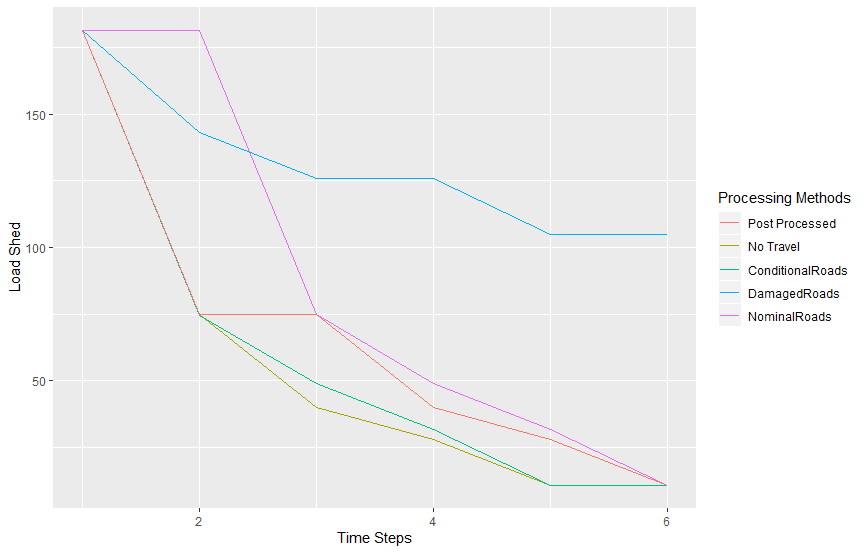
\includegraphics[width=.75\textwidth, %height=0.5\textheight,keepaspectratio]{Rplot37.png}

%\end{figure}
%\begin{figure}[H]
	%\centering
	%\caption{Load Shed by shift in the 30 bus case, recovery scenario 2}
	%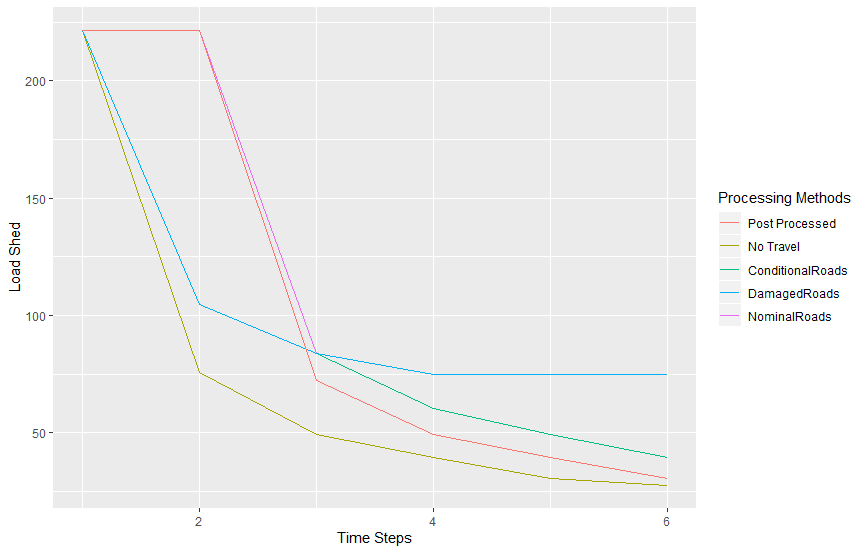
\includegraphics[width=.75\textwidth, %height=0.5\textheight,keepaspectratio]{Rplot30Scenario2.png}
	
%\end{figure}


\begin{figure}
	\centering
	\begin{subfigure}{.5\textwidth}
		\centering
		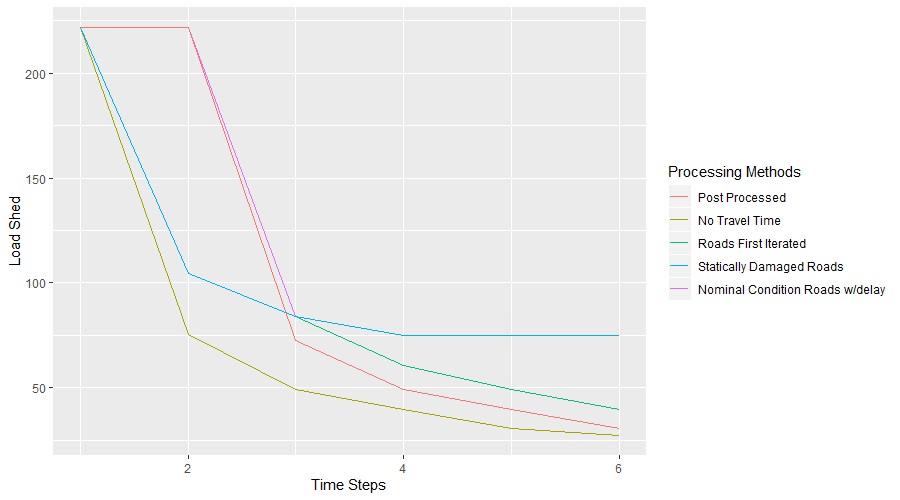
\includegraphics[width=.9\linewidth]{Rplot30Scenario2Fixed.png}
		\caption{Load Shed by shift in the 30 bus case\newline recovery scenario 2}
		\label{fig:sub1}
	\end{subfigure}%
	\begin{subfigure}{.5\textwidth}
		\centering
		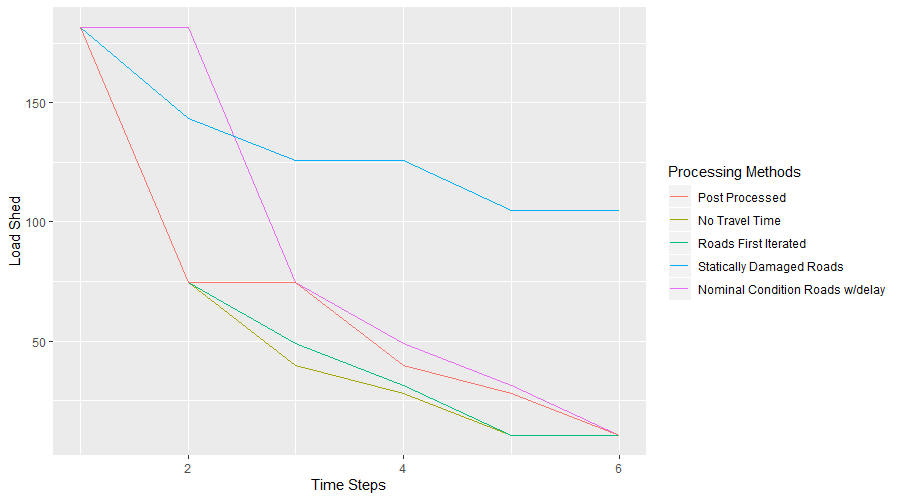
\includegraphics[width=.9\linewidth]{Rplot37Fixed.png}
		\caption{Load Shed by shift in the 30 bus case\newline recovery scenario 1}
		\label{fig:sub2}
	\end{subfigure}
	\caption{Comparisons of recovery on both 30 bus scenarios}
\end{figure}
The figures suggest that increased coordination between repair agencies improves the rate at which power can be restored. This is largely intuitive, but suggests that a revision in governmental or utility processes for handling post-disaster relief can result in more efficient recovery. The repair schedule generated from conditioning is closest to the lower bound in both scenarios (357.7 MW-shifts of unserviced demand vs 345.4 in the first scenario, 559.4 vs 444 in the higher damage scenario). The post-processed schedule presumes nominal road operation which would in practice mean that the power utility can dictate the road repair schedule and road clearing starts far enough ahead that any road needed by the power utility to affect repairs is traversable at its nominal runtime by the time it is needed. Given this, we conclude that coordinated repair is better than a best-case post processed schedule and is closer to the optimal way to treat the problem.
\subsection{IEEE 57 Bus Network}
 \vspace*{-12pt}
The setup for this case is nearly identical to the setup for the 30 bus case above, but with a different power grid in order to demonstrate that differences in repair schedules are not due to overfitting to a topology. The IEEE 57 bus network topology is another standard test network based on part of the American Electric Power System in the Midwestern US. Similar amounts of damage is applied to this network before the models were solved.

\begin{figure}[]
	\centering
	\caption{Load Shed by shift in the 57 bus case}
	\includegraphics[width=.5\textwidth, height=0.5\textheight,keepaspectratio]{RPlot57Fixed.png}
	
\end{figure}

Again we draw similar conclusions: More coordination once more leads to faster repairs of the power grid leading to lower total load shedding. The difference here is that the post-processed schedule with nominal condition roads is better than the conditioned solution method for one shift rather than being always better. That said, the iterated repair method still has a lower total demand loss over its planning horizon than the best possible case of the post processed schedule (936.8 vs 943.1 MW-shifts of unsatisfied power demand). These results are similar to both scenarios from the 30 bus case allowing us to conclude that solving road and power repair iteratively is better than trying to handle the power repair problem alone and the post-process into a valid repair schedule.
\section{\large{Conclusions and Future Research Directions}}
\label{sec:issues}
\vspace*{-12pt}

From this preliminary study, we draw the conclusion that increasing levels of model complexity which represent improved fidelity to fully coordinated operations yields lower levels of power load shedding. This suggests that at a practical level the agency responsible for restoration of the road grid should keep the agency responsible for the power grid informed of their plans as well as the state of the road network in order to more quickly restore power after a disaster.

Given these initial observations, we think that larger grids should be tackled in a future study to see if the results can be generalized to larger, more realistic size networks. Moreover, one can combine the preparedness and recovery phases of coordinated disaster logistics in a two-stage stochastic program to further optimize the disaster operations across road and power infrastructures.

\bibliographystyle{plain}
\bibliography{sources}

\end{document}
